\chapter{Resultados}
	
	\section{Diseño del sistema desalinizador}
		
		Después de un profundo análisis se logró un diseño modular vertical cuyos componentes principales se pueden observar en el~\cref{ch:dibujos-isométricos}. En la~\cref{fig:Sistema1} se puede contemplar el ensamblado propuesto.
		
		\begin{figure}[H]
			\centering
			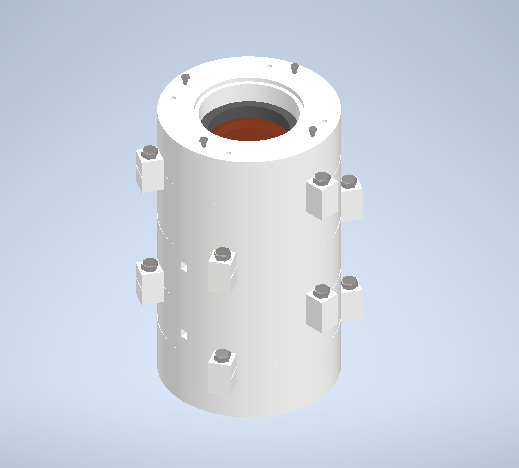
\includegraphics[
				width=\linewidth,
				height=70mm,
				keepaspectratio
			]{Resultados/Sistema/Sistema1.png}
			\caption{Propuesta del sistema desalinizador}
			\label{fig:Sistema1}
		\end{figure}
		
		En las secciones siguientes se detallarán los elementos que componen a este sistema, para lo cual se debe considerar que en las imágenes siguientes el etiquetado \textbf{T} hace referencia a las uniones con tornillos y el etiquetado \textbf{A} al espacio designado para el aislante térmico.
	
		\subsection{Contenedor de agua de mar}
			
			Su función básica es contener el agua a desalinizar y servir al mismo tiempo como depósito para la retroalimentación del sistema. Los elementos principales etiquetados en la \cref{fig:Contenedor-agua-mar-corte-1} se detallan a continuación: 1) Entrada del suministro de agua. 2) Orificio de succión para la entrada a la bomba peristáltica. 3) Orificio para la tubería conectada a la salida de la bomba peristáltica. 4) Canales de retroalimentación provenientes de la cámara de evaporación.
		
			\begin{figure}[H]
				\centering
				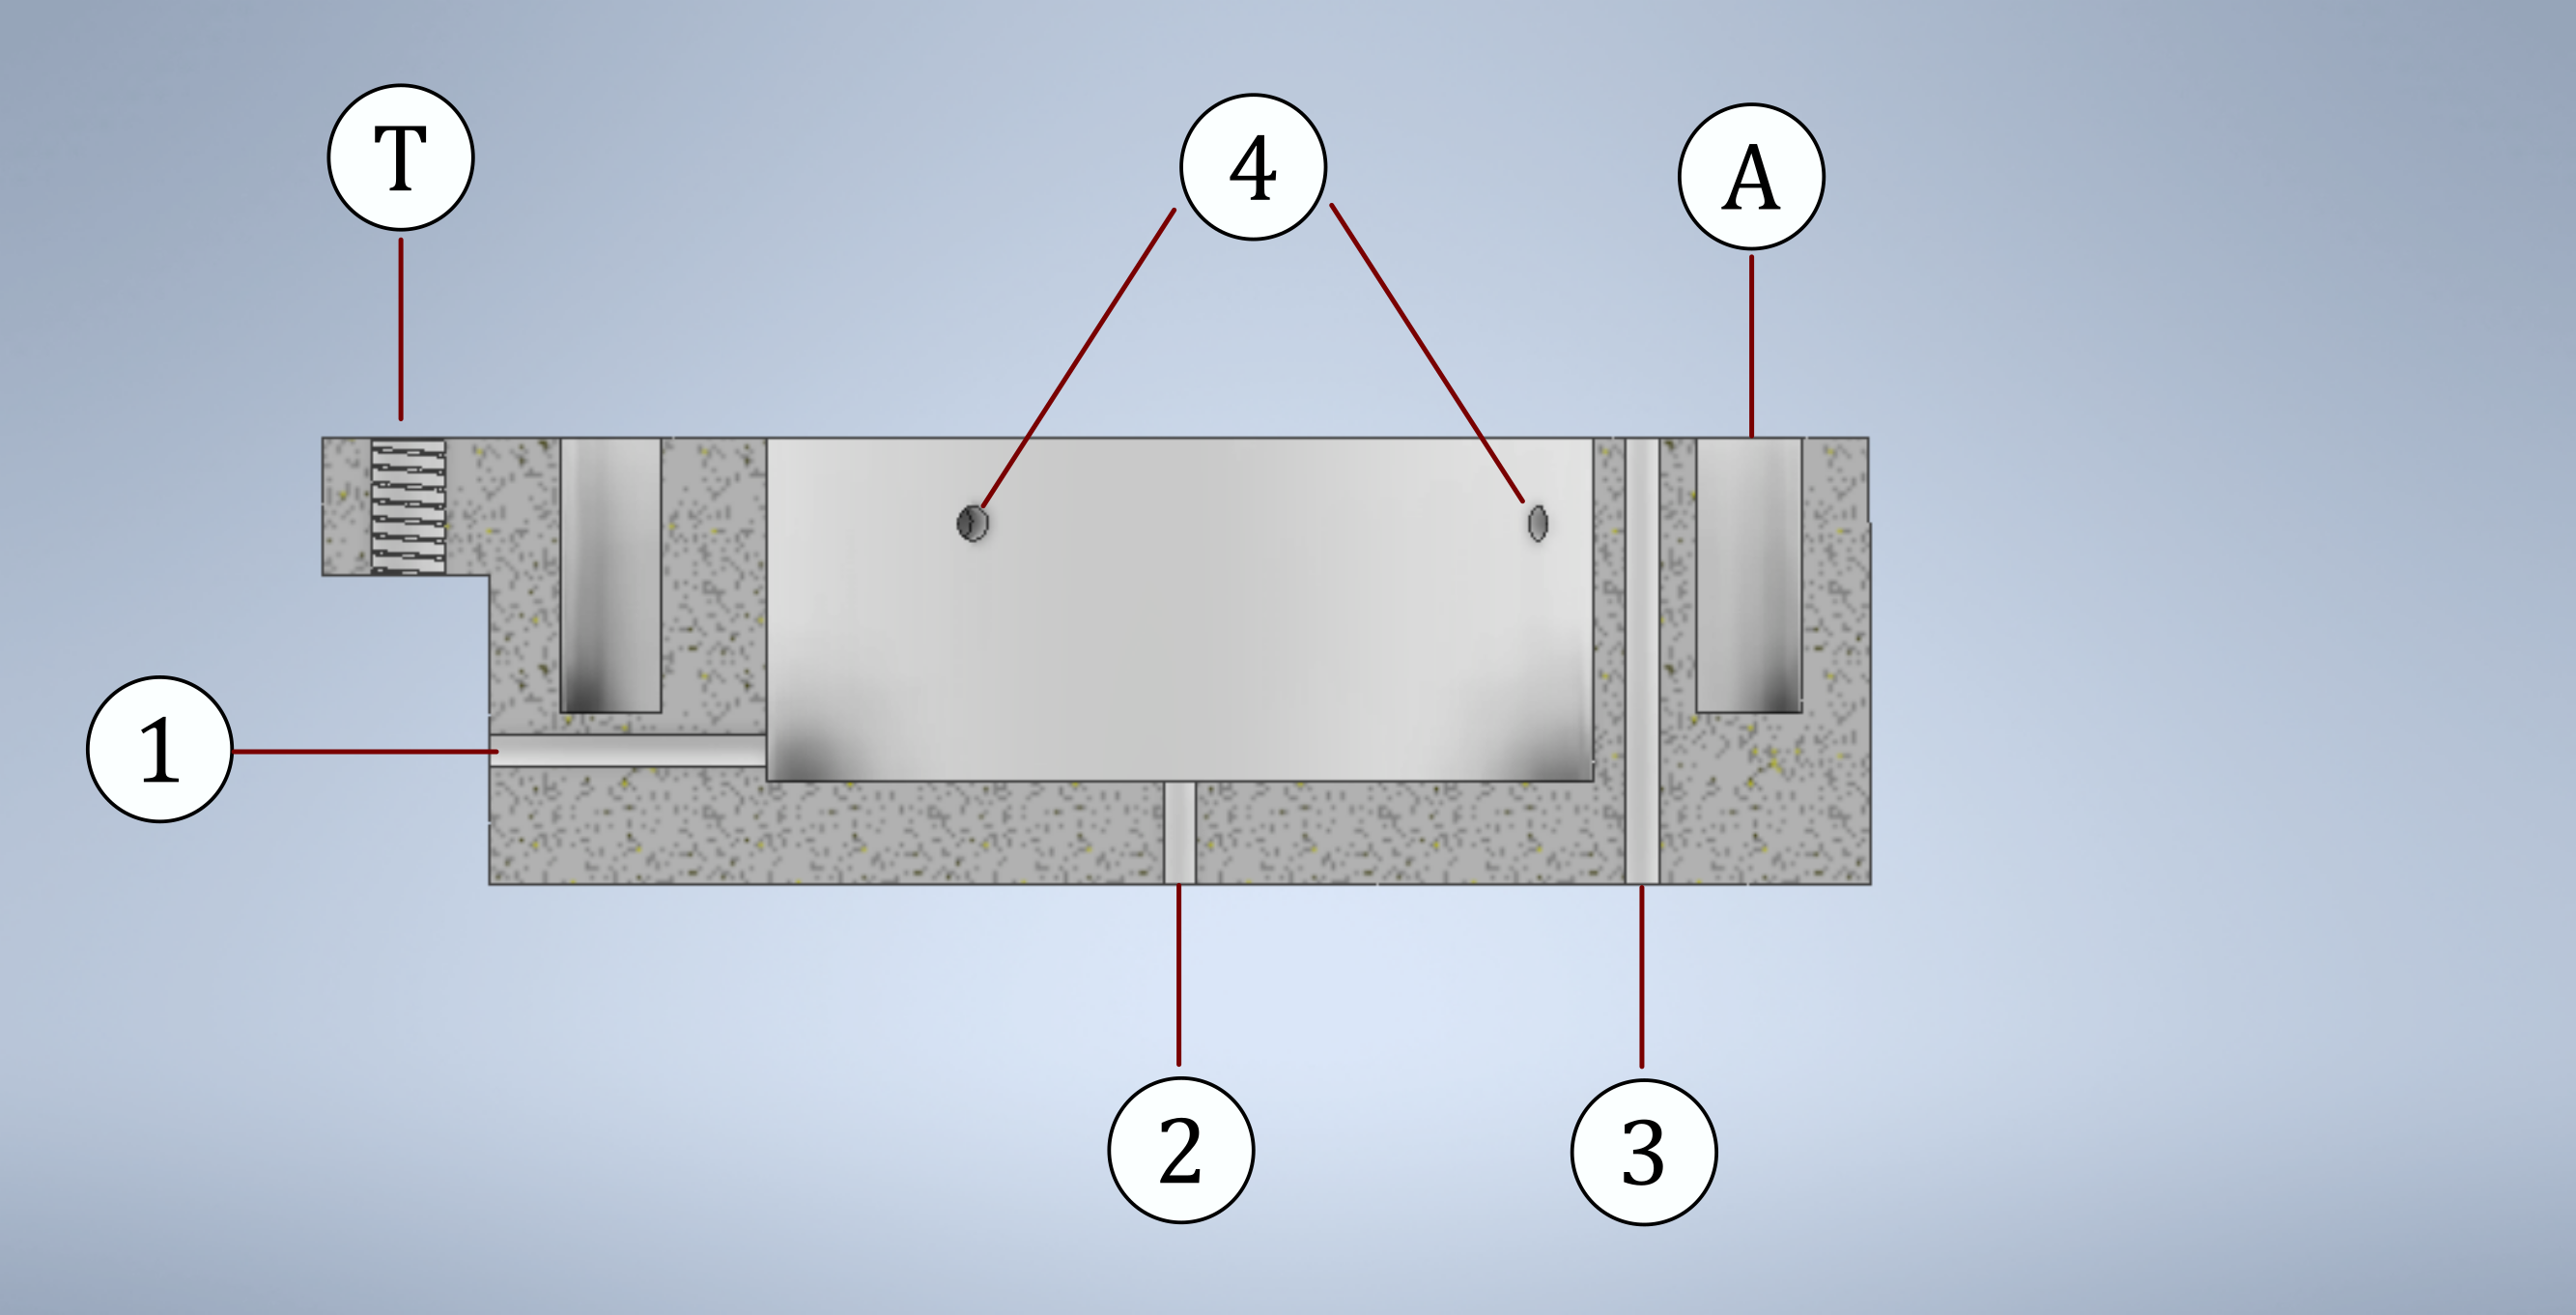
\includegraphics[
					width=\linewidth,
					height=70mm,
					keepaspectratio
				]{Resultados/Cortes/Contenedor-agua-mar-corte-1.png}
				\caption{Contenedor de agua de mar. Corte 1}
				\label{fig:Contenedor-agua-mar-corte-1}
			\end{figure}
		
		\subsection{Contenedor de agua destilada}
			
			Su función básica es contener el agua a desalinizada y promover la condensación del vapor con intercambio de calor entre la misma cámara y la de agua de mar. Los elementos principales etiquetados en las \cref{fig:Contenedor-agua-destilada-corte-1,fig:Contenedor-agua-destilada-corte-2} se detallan a continuación: 1) Entrada de vapor. 2) Salida de agua altamente salina proveniente de la cámara. 3) Salida de agua destilada. 4) Continuación del canal de alimentación hacia la cámara de concentración. I) Roscado para el intercambiador de calor propuesto.
		
			\begin{figure}[H]
				\centering
				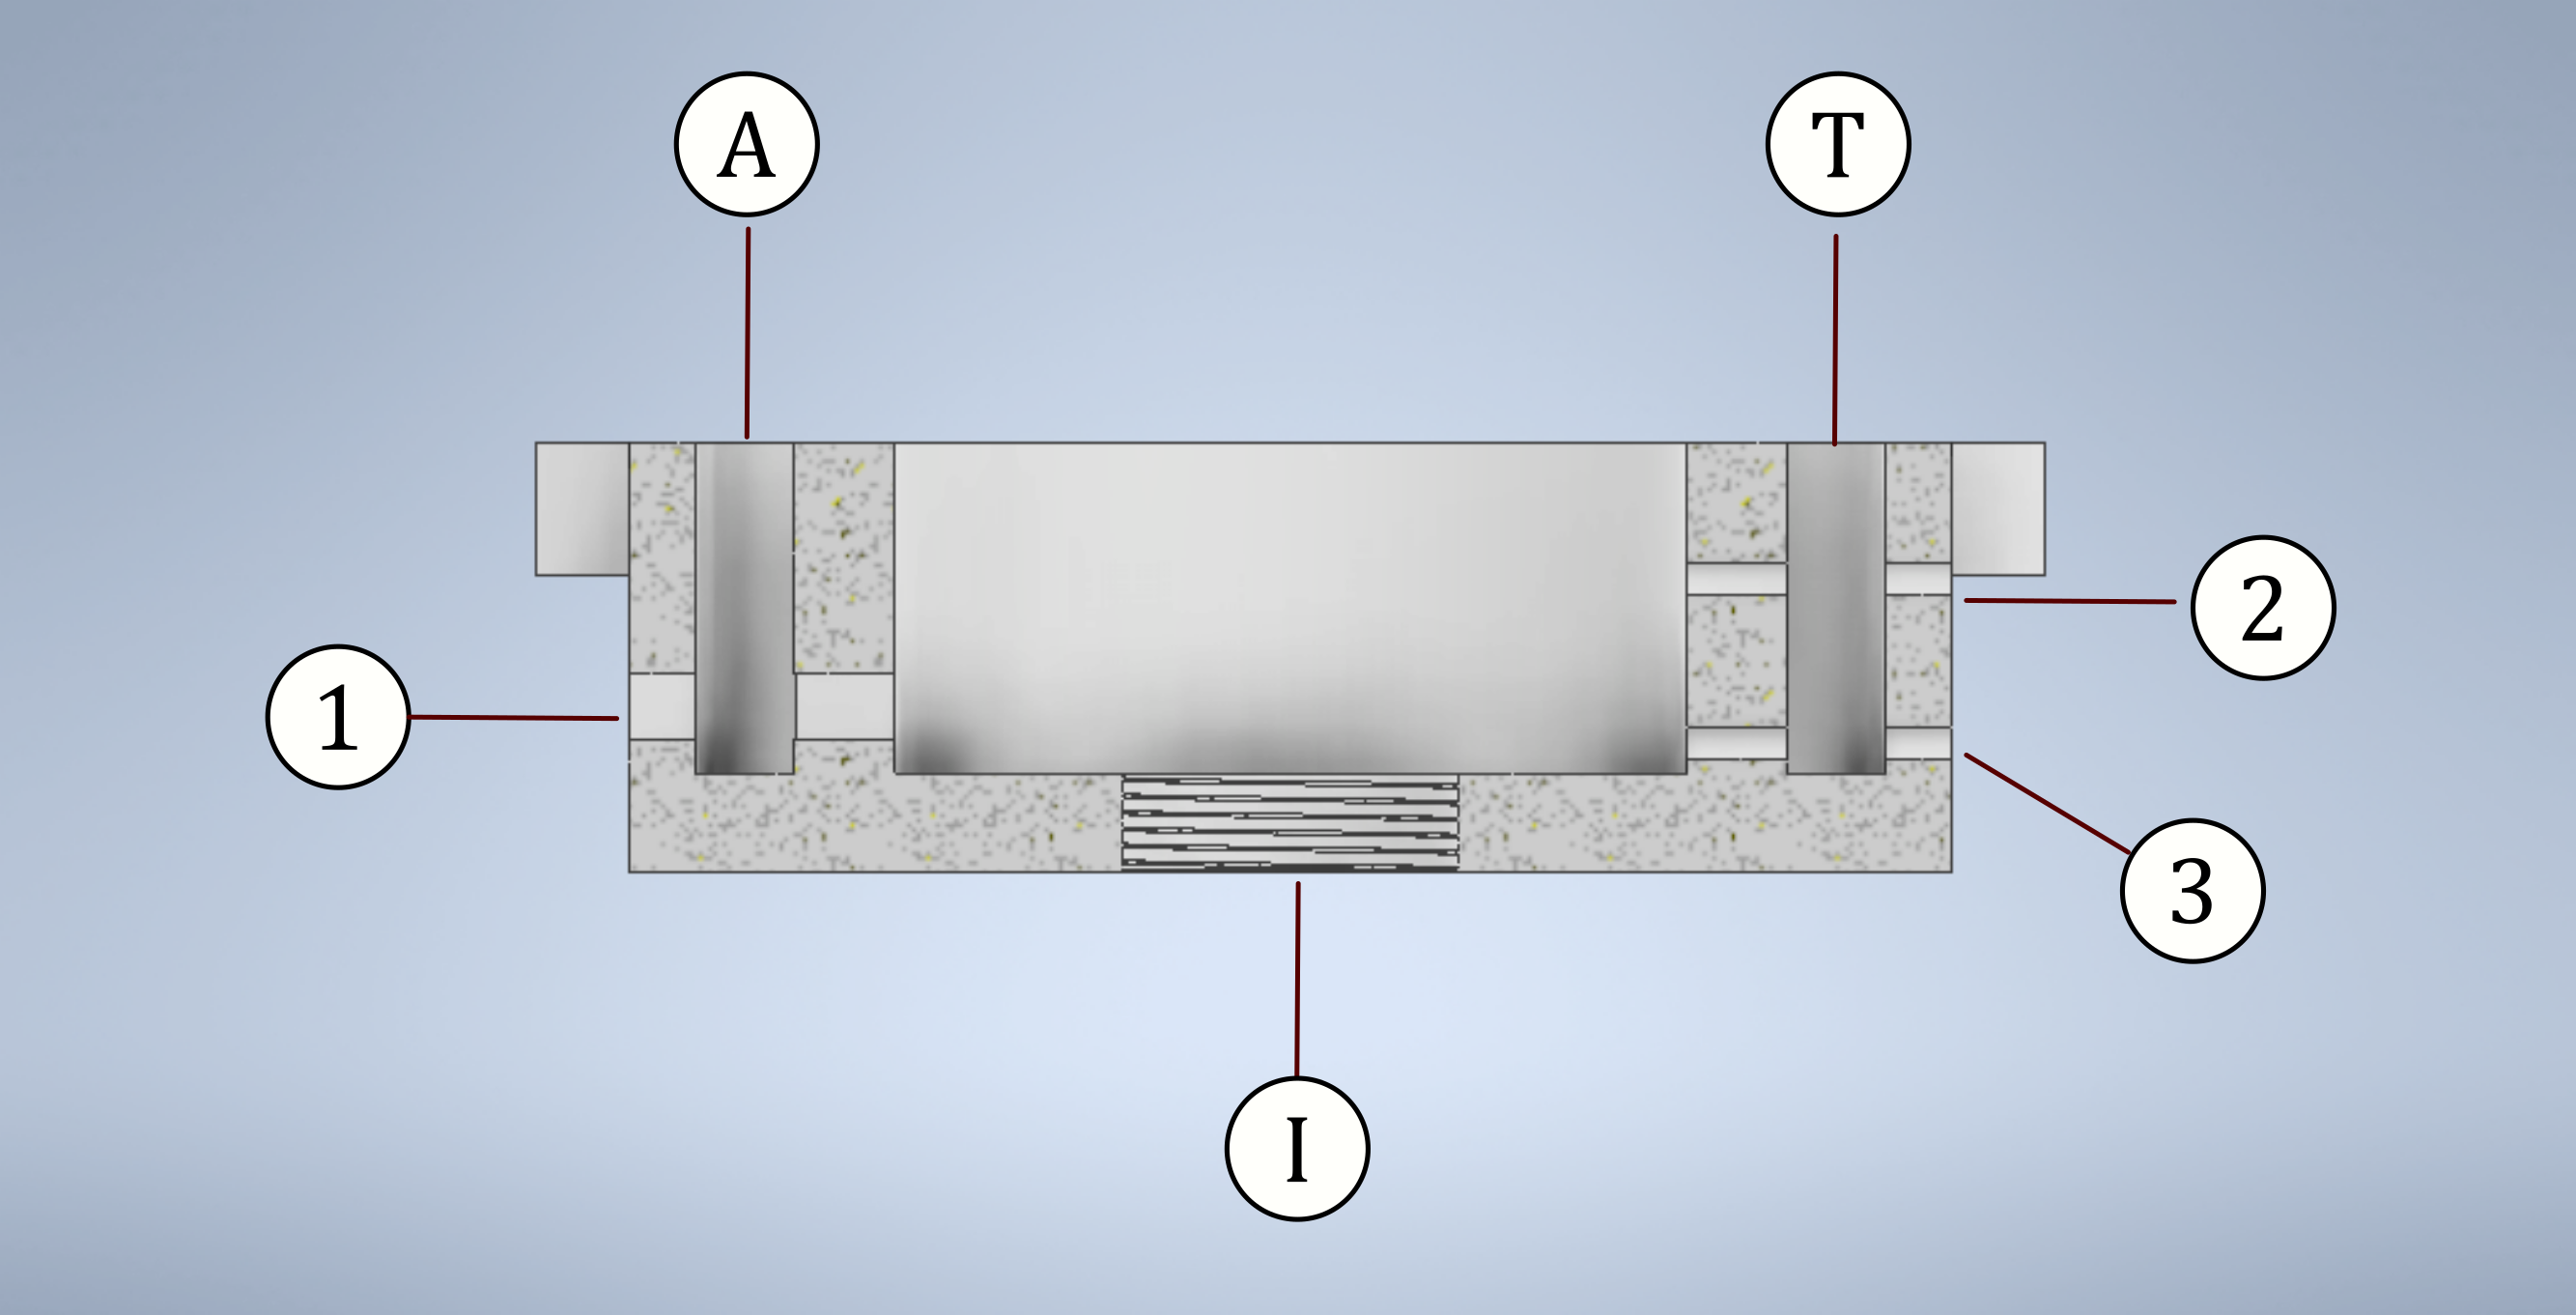
\includegraphics[
					width=\linewidth,
					height=70mm,
					keepaspectratio
				]{Resultados/Cortes/Contenedor-agua-destilada-corte-1.png}
				\caption{Contenedor de agua destilada. Corte 1}
				\label{fig:Contenedor-agua-destilada-corte-1}
			\end{figure}
			
			\begin{figure}[H]
				\centering
				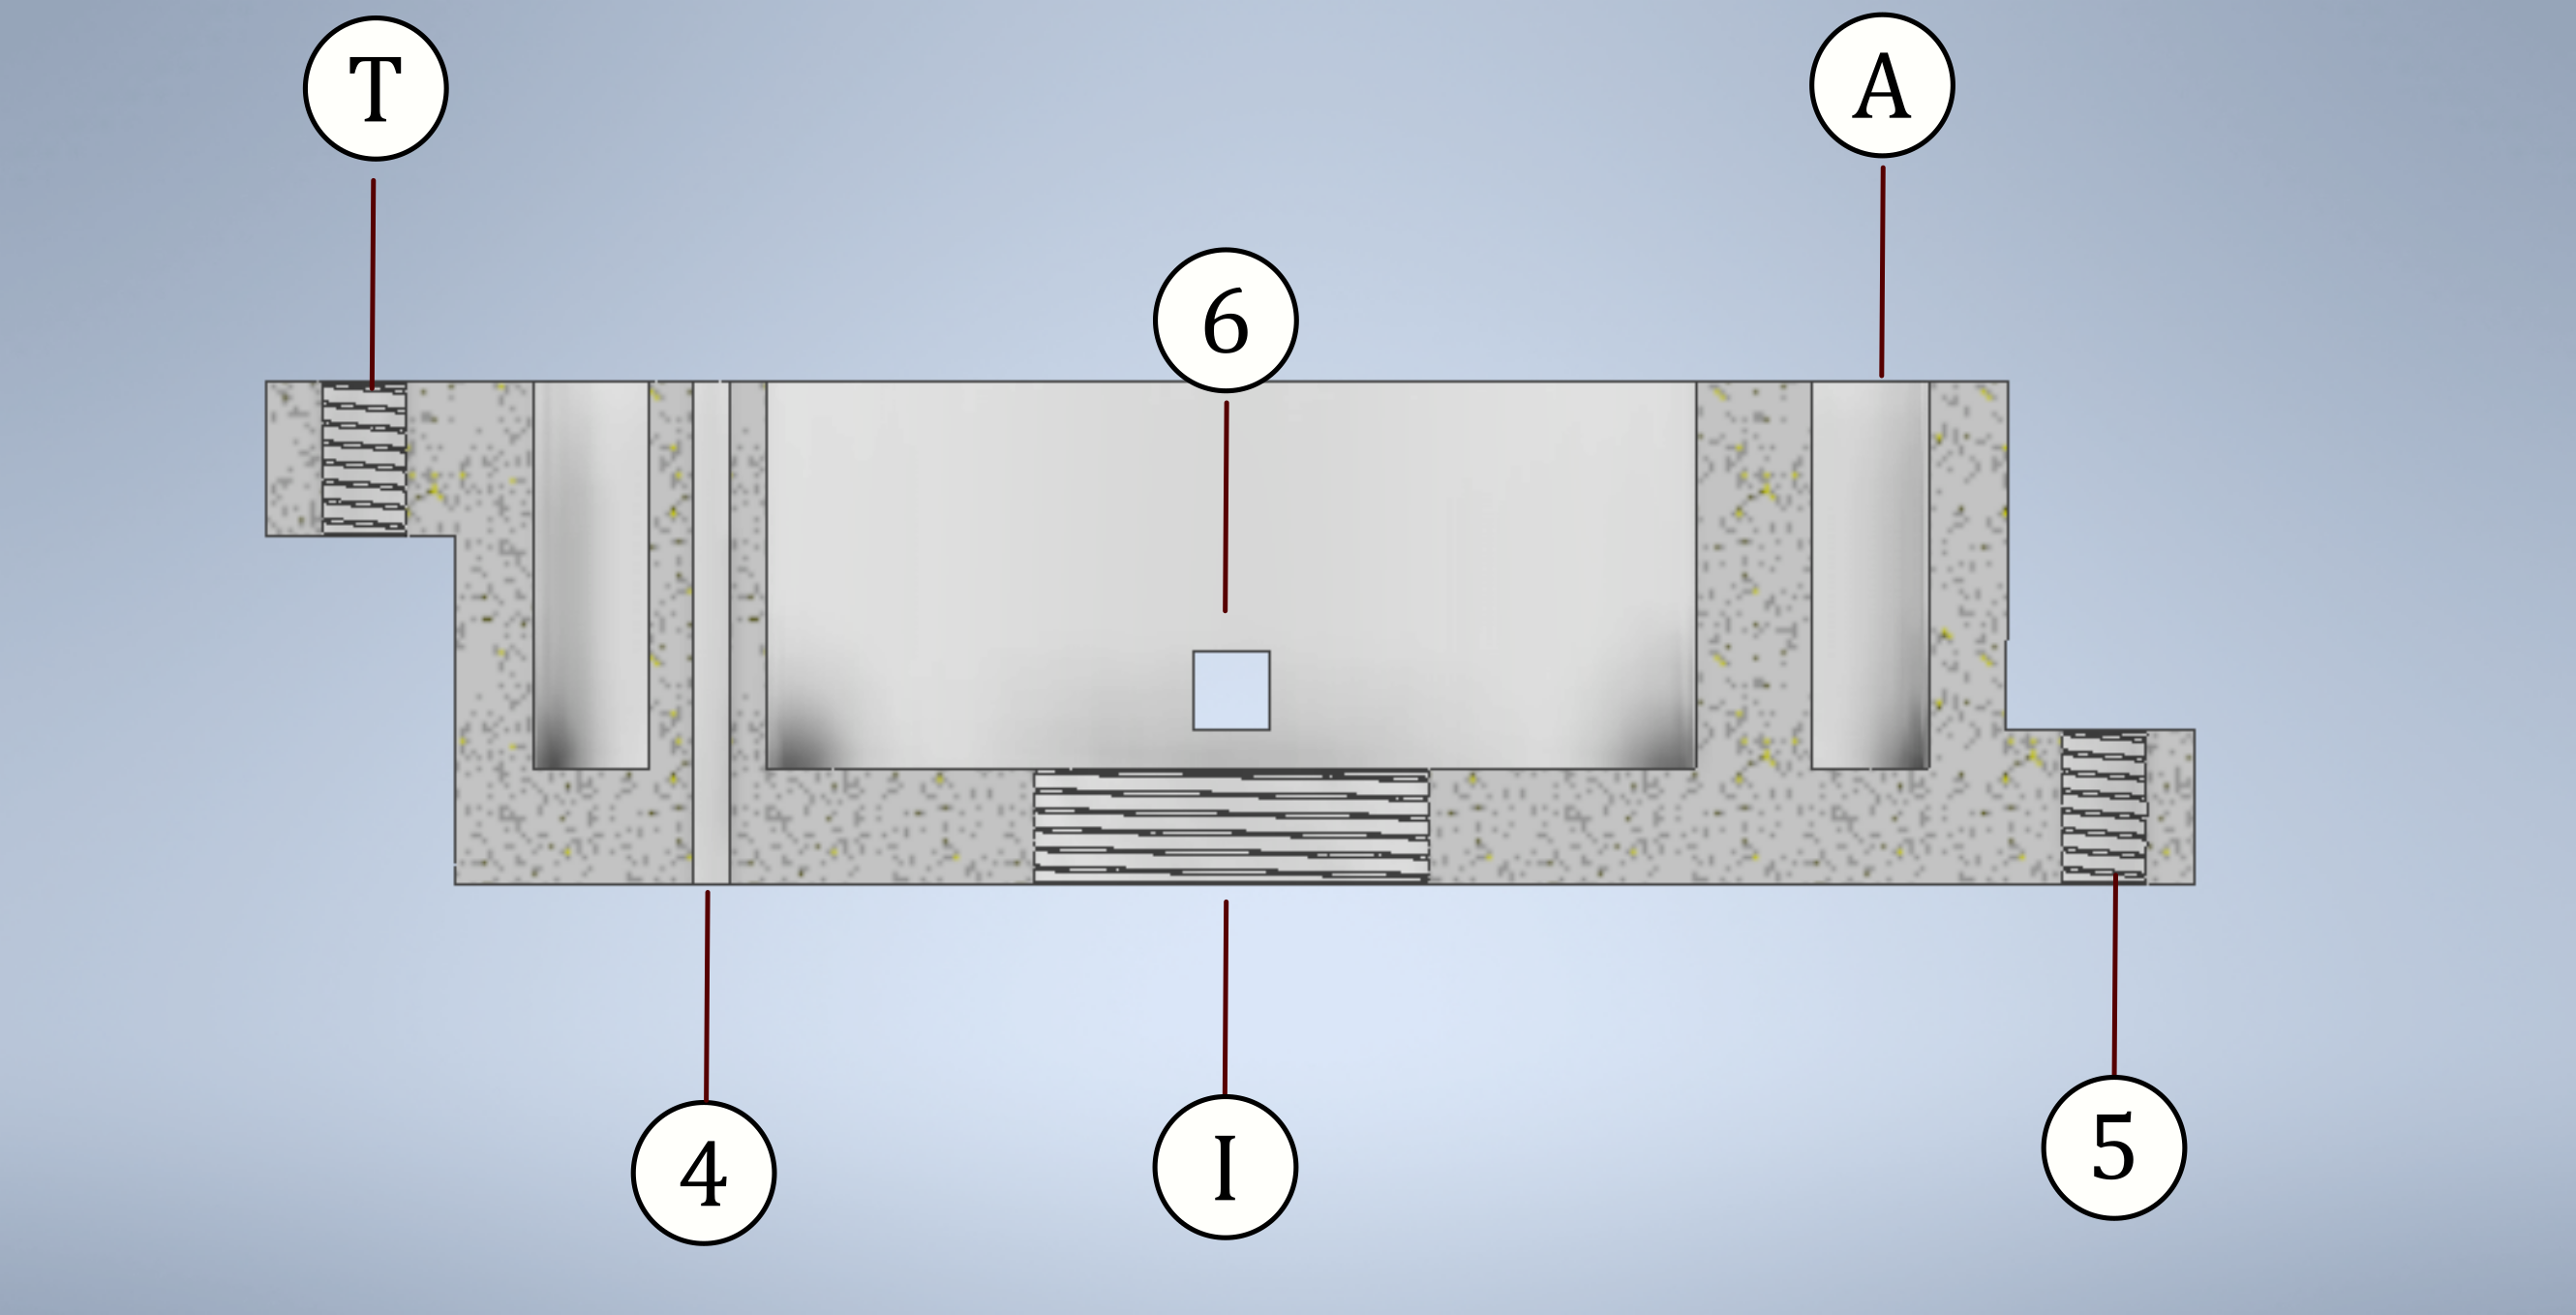
\includegraphics[
					width=\linewidth,
					height=70mm,
					keepaspectratio
				]{Resultados/Cortes/Contenedor-agua-destilada-corte-2.png}
				\caption{Contenedor de agua destilada. Corte 2}
				\label{fig:Contenedor-agua-destilada-corte-2}
			\end{figure}
			
			Aunque no se observa en los cortes sugeridos, en las paredes de la cámara se encuentra la continuación de los canales de retroalimentación entre la cámara de evaporación y la cámara de agua de mar. Los detalles se pueden observar en el dibujo isométrico disponible en el~\cref{ch:dibujos-isométricos}.
			
		\subsection{Cámara de evaporación}
			
			Su función básica es favorecer el proceso de evaporación aumentando el área superficial por unidad de volumen del agua de mar a su vez de mantener retroalimentación por gravedad hacia la cámara de agua de mar. Los elementos principales etiquetados en las \cref{fig:camara-evaporación-corte-1,fig:camara-evaporación-corte-2} se detallan a continuación: 1) Salida de agua altamente salina 2) Continuación del canal de alimentación hacia la cámara de concentración. 3) Salida de vapor hacia la cámara de condensado. D) Canales de desagüe para evitar la acumulación de agua salina.
		
			\begin{figure}[H]
				\centering
				\includegraphics[
					width=\linewidth,
					height=70mm,
					keepaspectratio
				]{Resultados/Cortes/camara-evaporación-corte-1.png}
				\caption{Cámara de evaporación. Corte 1}
				\label{fig:camara-evaporación-corte-1}
			\end{figure}
			
			\begin{figure}[H]
				\centering
				\includegraphics[
					width=\linewidth,
					height=70mm,
					keepaspectratio
				]{Resultados/Cortes/camara-evaporación-corte-2.png}
				\caption{Cámara de evaporación. Corte 2}
				\label{fig:camara-evaporación-corte-2}
			\end{figure}
			
		\subsection{Cámara de concentración}
			
			\subsubsection{Parte inferior}
				
				Su función básica es favorecer el proceso de evaporación aumentando el área superficial por unidad de volumen del agua de mar a su vez de mantener retroalimentación por gravedad hacia la cámara de agua de mar. Los elementos principales etiquetados en las \cref{fig:Arena-concentrador-corte-1,fig:Arena-concentrador-corte-2} se detallan a continuación: 1) Entrada del agua de mar. 2) Salida del agua de mar.
			
				\begin{figure}[H]
					\centering
					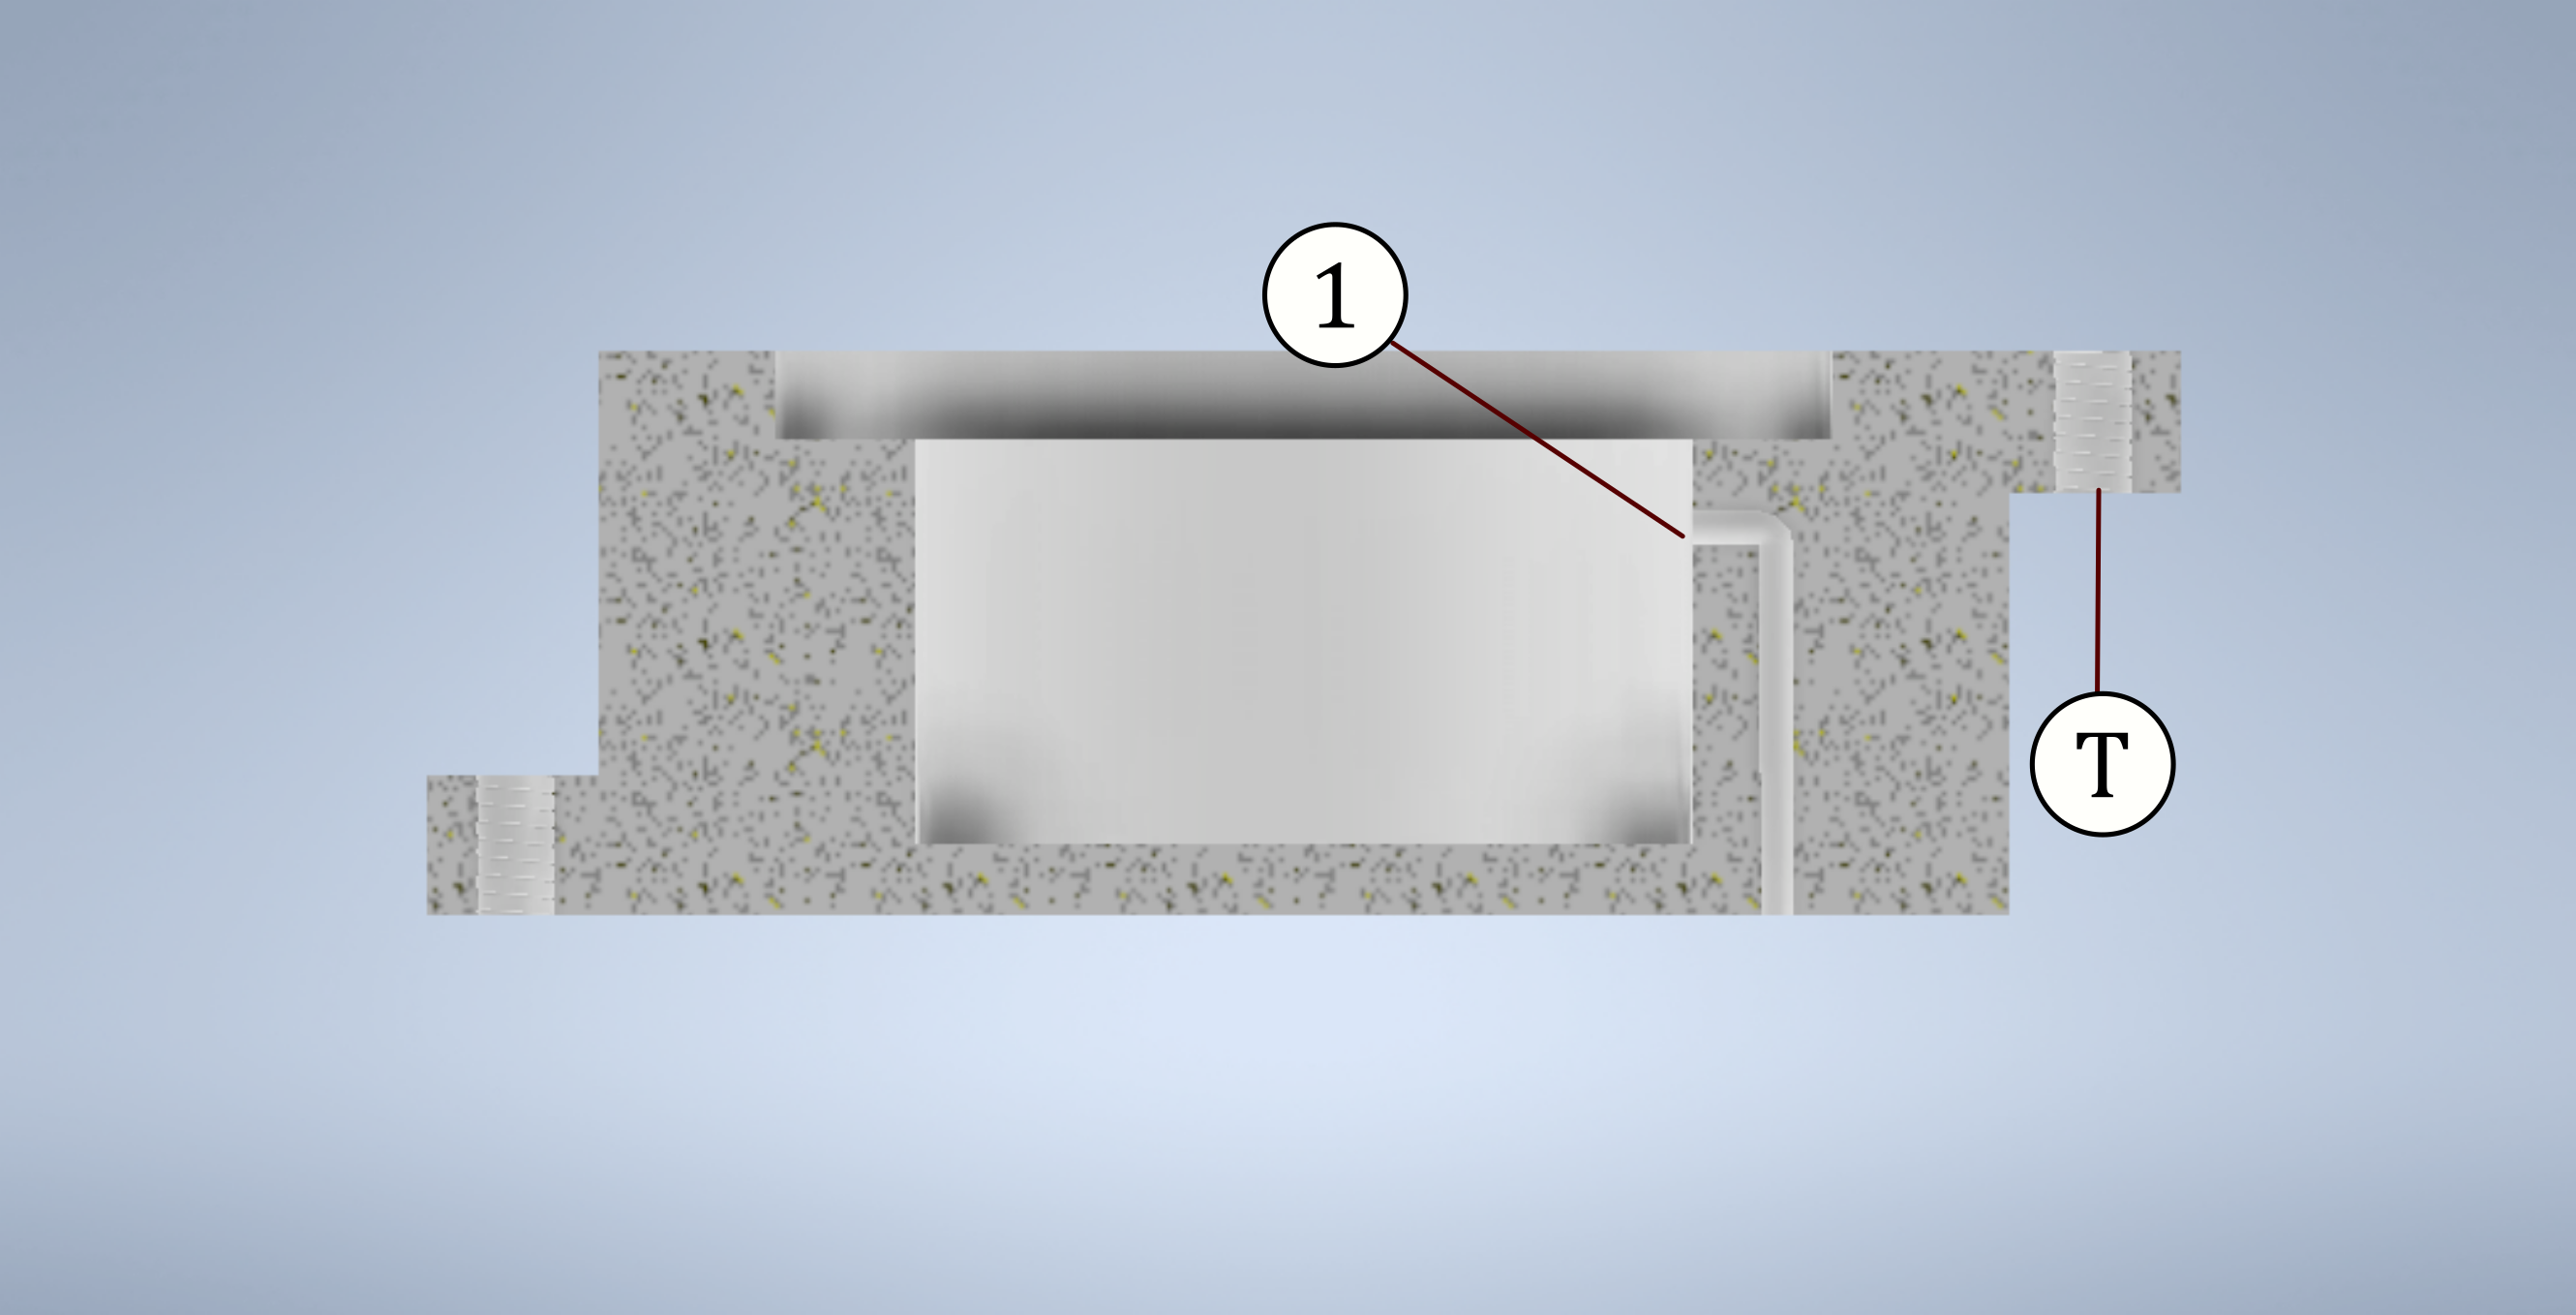
\includegraphics[
						width=\linewidth,
						height=70mm,
						keepaspectratio
					]{Resultados/Cortes/Arena-concentrador-corte-1.png}
					\caption{Cámara de concentración; parte inferior. Corte 1}
					\label{fig:Arena-concentrador-corte-1}
				\end{figure}
				
				\begin{figure}[H]
					\centering
					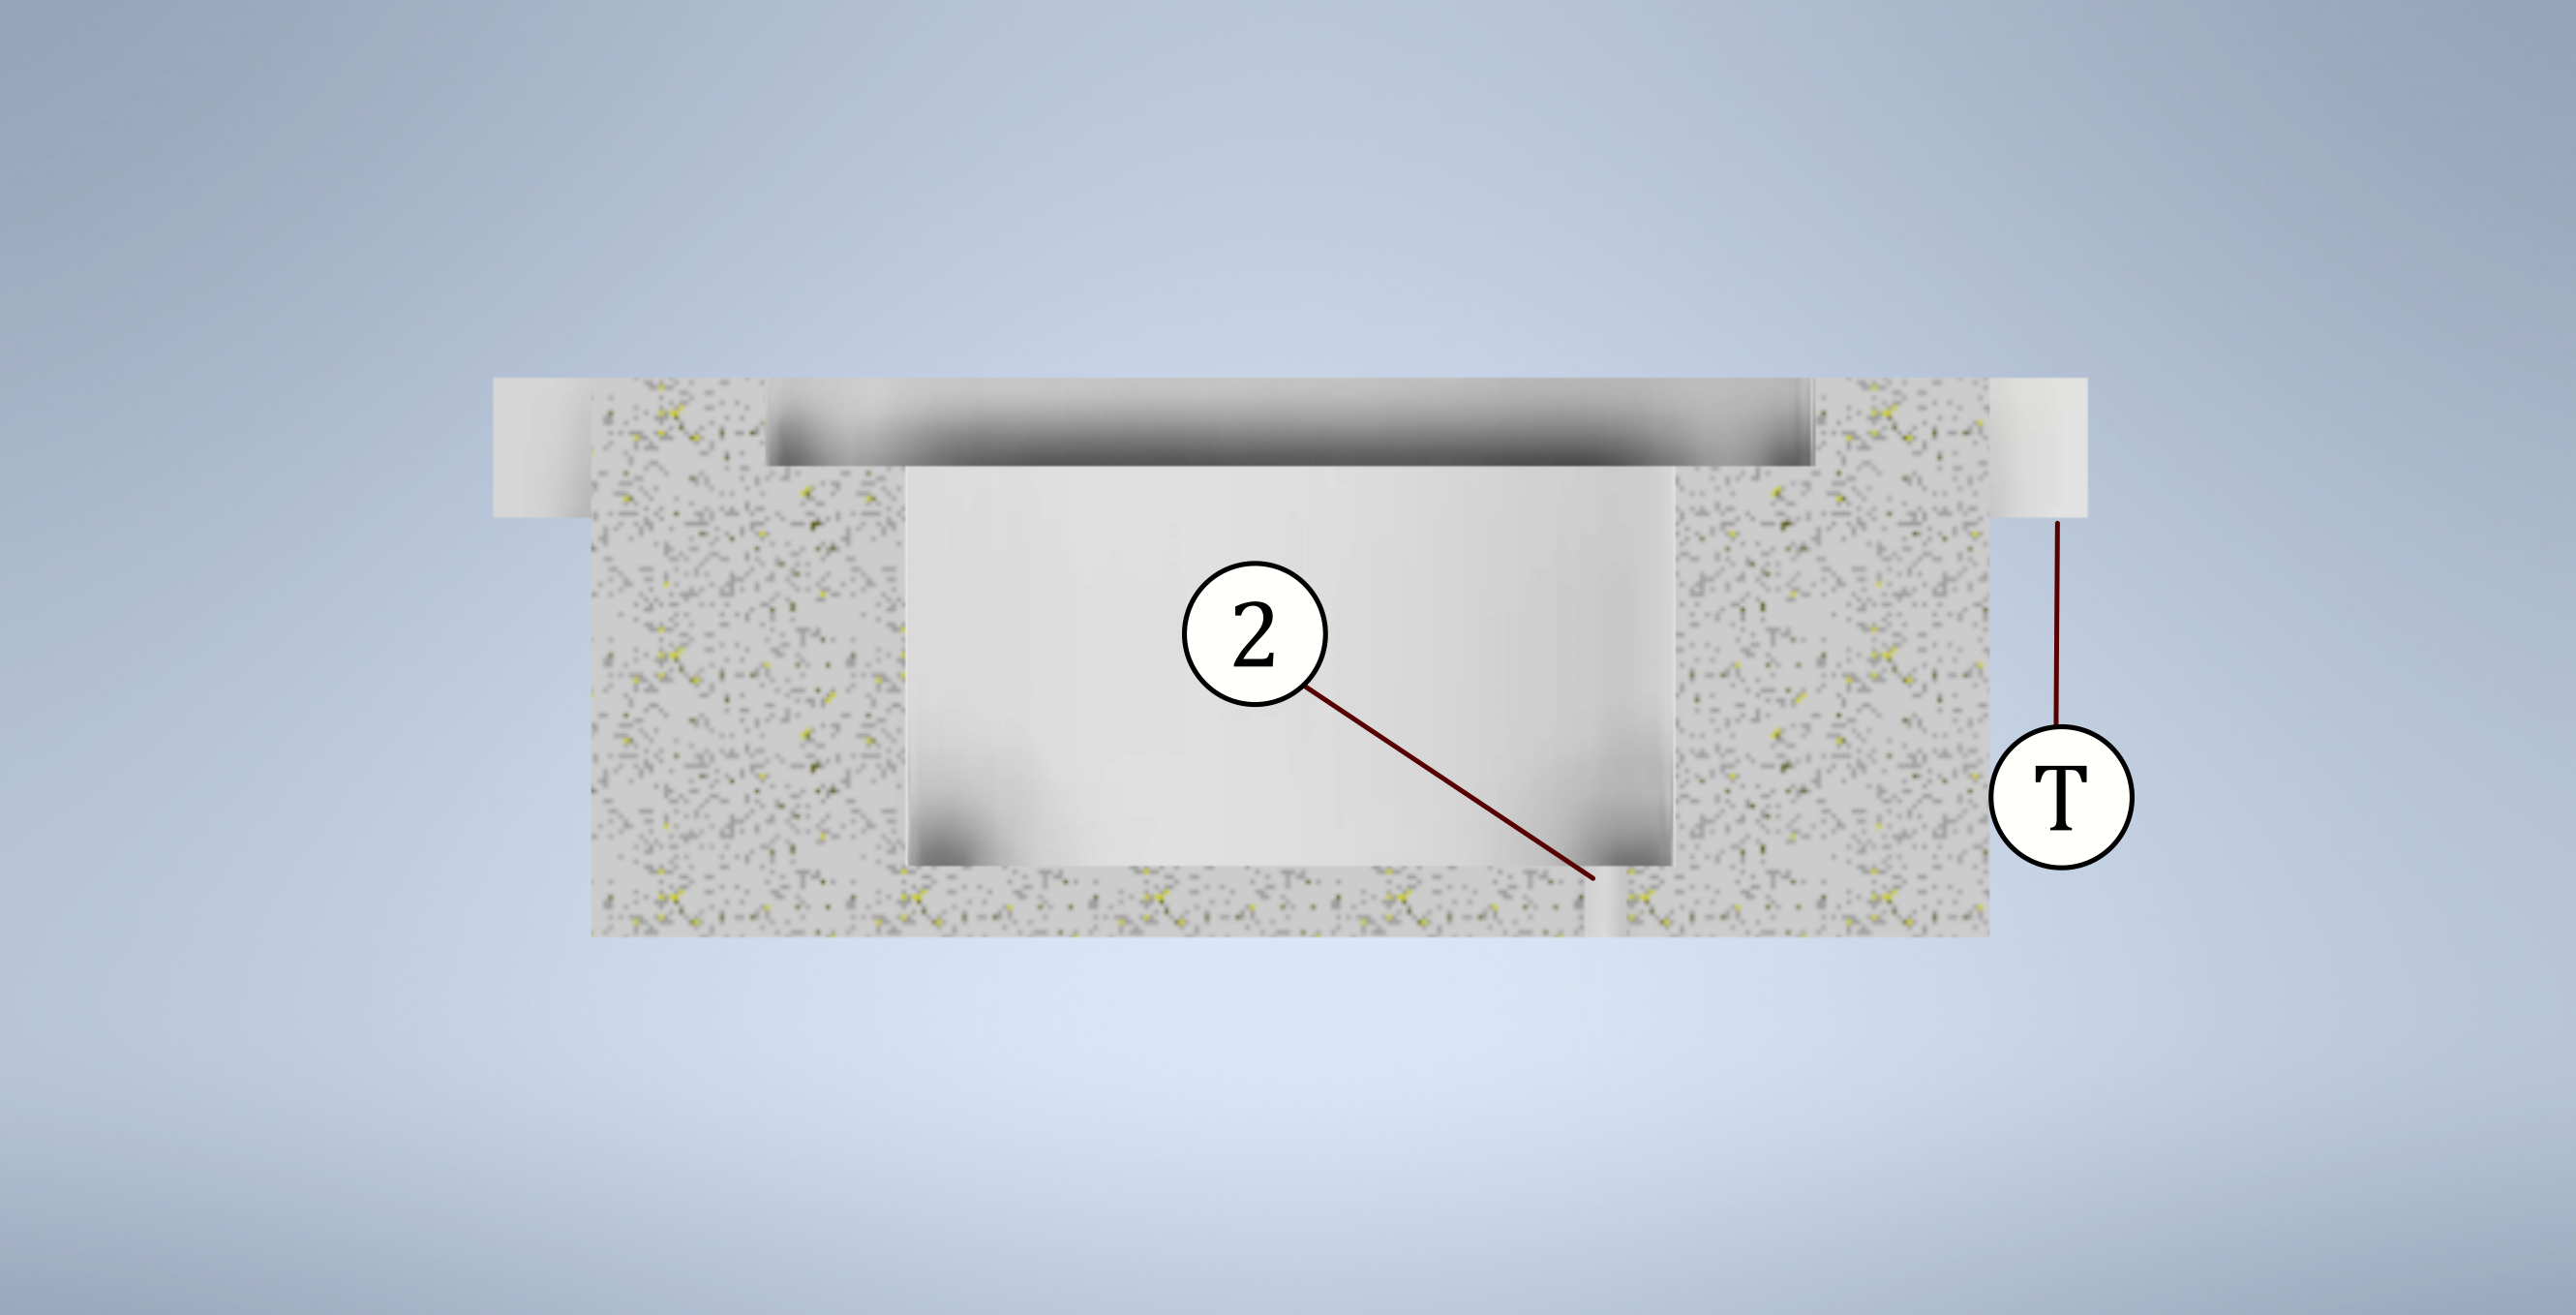
\includegraphics[
						width=\linewidth,
						height=70mm,
						keepaspectratio
					]{Resultados/Cortes/Arena-concentrador-corte-2.png}
					\caption{Cámara de concentración; parte inferior. Corte 2}
					\label{fig:Arena-concentrador-corte-2}
				\end{figure}
			
			\subsubsection{Parte superior}
				
				La parte superior de la cámara de concentración consta de la tapa que ayuda a la de sujeción del cristal de cuarzo y el recibidor solar. Estos se unen a la cámara inferior
			
			
%			\begin{figure}
%				\centering
%				\includegraphics[
%					width=\linewidth,
%					keepaspectratio
%				]{dsf}
%			\end{figure}
%		
%		Conductividad térmica
%		
%		Para conocer $\gls{cs}_{\text{agua}}$ de la \cref{table:Conductividad-térmica-agua-salada} se usa \eqref{equ:interpolación-lineal-simple} para obtener la conductividad estimada a los \qty{13}{\degreeCelsius} y a los \qty{94.7}{\degreeCelsius}.
%		
%		\begin{align*}
%			\gls{cs}_{13} &= \qty{0.586}{\watt\per\m\kelvin} + \dfrac{\qty{0.601}{\watt\per\m\kelvin} - \qty{0.586}{\watt\per\m\kelvin}}{\qty{20}{\degreeCelsius}-\qty{10}{\degreeCelsius}} \times (\qty{20}{\degreeCelsius} - \qty{13}{\degreeCelsius})\\
%			\gls{cs}_{13} &= \qty{0.591}{\watt\per\m\kelvin}\\
%			\gls{cs}_{94.7} &= \qty{0.670}{\watt\per\m\kelvin} + \dfrac{\qty{0.674}{\watt\per\m\kelvin} - \qty{0.670}{\watt\per\m\kelvin}}{\qty{100}{\degreeCelsius}-\qty{90}{\degreeCelsius}} \times (\qty{100}{\degreeCelsius} - \qty{94.7}{\degreeCelsius})\\
%			\gls{cs}_{94.7} &= \qty{0.672}{\watt\per\m\kelvin}
%		\end{align*}
%		
%		Una vez obtenidos sacamos el promedio incluyendo el resto del intervalo dándonos que:
%		\begin{equation*}
%			\gls{cs}_{\text{agua}} = \qty{0.638}{\watt\per\m\kelvin}
%		\end{equation*}